\hypertarget{vec_8c}{
\section{/home/mgh/LanlGeoMag/libLanlGeoMag/vec.c File Reference}
\label{vec_8c}\index{/home/mgh/LanlGeoMag/libLanlGeoMag/vec.c@{/home/mgh/LanlGeoMag/libLanlGeoMag/vec.c}}
}
{\tt \#include $<$math.h$>$}\par
{\tt \#include \char`\"{}Lgm/LgmVec.h\char`\"{}}\par


Include dependency graph for vec.c:\nopagebreak
\begin{figure}[H]
\begin{center}
\leavevmode
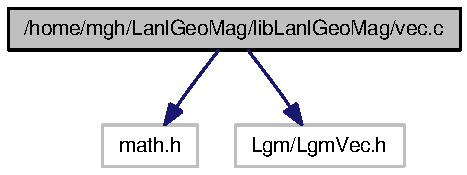
\includegraphics[width=130pt]{vec_8c__incl}
\end{center}
\end{figure}
\subsection*{Functions}
\begin{CompactItemize}
\item 
void \hyperlink{vec_8c_390e6254a5488b560011b0c1880745dd}{Lgm\_\-CrossProduct} (\hyperlink{struct_lgm___vector}{Lgm\_\-Vector} $\ast$a, \hyperlink{struct_lgm___vector}{Lgm\_\-Vector} $\ast$b, \hyperlink{struct_lgm___vector}{Lgm\_\-Vector} $\ast$c)
\item 
double \hyperlink{vec_8c_bc4f50854f167ab190d1ec48cba5fb6f}{Lgm\_\-DotProduct} (\hyperlink{struct_lgm___vector}{Lgm\_\-Vector} $\ast$a, \hyperlink{struct_lgm___vector}{Lgm\_\-Vector} $\ast$b)
\item 
double \hyperlink{vec_8c_851c60a1429e5b2d8bc5feb2d59af700}{Lgm\_\-NormalizeVector} (\hyperlink{struct_lgm___vector}{Lgm\_\-Vector} $\ast$a)
\item 
void \hyperlink{vec_8c_eb74ea961a602bfdb729ade5b1282946}{Lgm\_\-ScaleVector} (\hyperlink{struct_lgm___vector}{Lgm\_\-Vector} $\ast$a, double value)
\item 
double \hyperlink{vec_8c_84b4b9aa2d74211cb12654e6be70cb82}{Lgm\_\-Magnitude} (\hyperlink{struct_lgm___vector}{Lgm\_\-Vector} $\ast$a)
\item 
void \hyperlink{vec_8c_47c6f330f5c1228f812b005094b64dfd}{Lgm\_\-ForceMagnitude} (\hyperlink{struct_lgm___vector}{Lgm\_\-Vector} $\ast$a, double mag)
\item 
void \hyperlink{vec_8c_d6b4ead73e36f4f3f77cc62bc88555d3}{Lgm\_\-MatTimesVec} (double A\mbox{[}3\mbox{]}\mbox{[}3\mbox{]}, \hyperlink{struct_lgm___vector}{Lgm\_\-Vector} $\ast$V, \hyperlink{struct_lgm___vector}{Lgm\_\-Vector} $\ast$Result)
\item 
void \hyperlink{vec_8c_2afeb786399b91dc38ba78adc88db1ce}{Lgm\_\-MatTimeMat} (double A\mbox{[}3\mbox{]}\mbox{[}3\mbox{]}, double B\mbox{[}3\mbox{]}\mbox{[}3\mbox{]}, double Result\mbox{[}3\mbox{]}\mbox{[}3\mbox{]})
\end{CompactItemize}


\subsection{Function Documentation}
\hypertarget{vec_8c_390e6254a5488b560011b0c1880745dd}{
\index{vec.c@{vec.c}!Lgm\_\-CrossProduct@{Lgm\_\-CrossProduct}}
\index{Lgm\_\-CrossProduct@{Lgm\_\-CrossProduct}!vec.c@{vec.c}}
\subsubsection[{Lgm\_\-CrossProduct}]{\setlength{\rightskip}{0pt plus 5cm}void Lgm\_\-CrossProduct ({\bf Lgm\_\-Vector} $\ast$ {\em a}, \/  {\bf Lgm\_\-Vector} $\ast$ {\em b}, \/  {\bf Lgm\_\-Vector} $\ast$ {\em c})}}
\label{vec_8c_390e6254a5488b560011b0c1880745dd}




Definition at line 7 of file vec.c.

Here is the caller graph for this function:\nopagebreak
\begin{figure}[H]
\begin{center}
\leavevmode
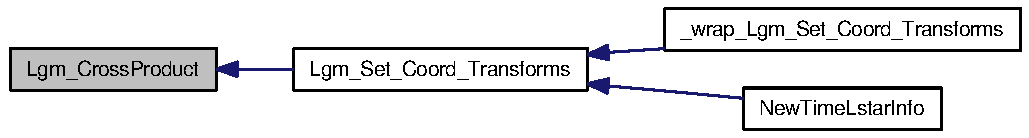
\includegraphics[width=265pt]{vec_8c_390e6254a5488b560011b0c1880745dd_icgraph}
\end{center}
\end{figure}
\hypertarget{vec_8c_bc4f50854f167ab190d1ec48cba5fb6f}{
\index{vec.c@{vec.c}!Lgm\_\-DotProduct@{Lgm\_\-DotProduct}}
\index{Lgm\_\-DotProduct@{Lgm\_\-DotProduct}!vec.c@{vec.c}}
\subsubsection[{Lgm\_\-DotProduct}]{\setlength{\rightskip}{0pt plus 5cm}double Lgm\_\-DotProduct ({\bf Lgm\_\-Vector} $\ast$ {\em a}, \/  {\bf Lgm\_\-Vector} $\ast$ {\em b})}}
\label{vec_8c_bc4f50854f167ab190d1ec48cba5fb6f}




Definition at line 18 of file vec.c.

Here is the caller graph for this function:\nopagebreak
\begin{figure}[H]
\begin{center}
\leavevmode
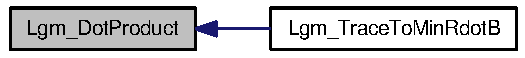
\includegraphics[width=144pt]{vec_8c_bc4f50854f167ab190d1ec48cba5fb6f_icgraph}
\end{center}
\end{figure}
\hypertarget{vec_8c_851c60a1429e5b2d8bc5feb2d59af700}{
\index{vec.c@{vec.c}!Lgm\_\-NormalizeVector@{Lgm\_\-NormalizeVector}}
\index{Lgm\_\-NormalizeVector@{Lgm\_\-NormalizeVector}!vec.c@{vec.c}}
\subsubsection[{Lgm\_\-NormalizeVector}]{\setlength{\rightskip}{0pt plus 5cm}double Lgm\_\-NormalizeVector ({\bf Lgm\_\-Vector} $\ast$ {\em a})}}
\label{vec_8c_851c60a1429e5b2d8bc5feb2d59af700}




Definition at line 27 of file vec.c.

Here is the caller graph for this function:\nopagebreak
\begin{figure}[H]
\begin{center}
\leavevmode
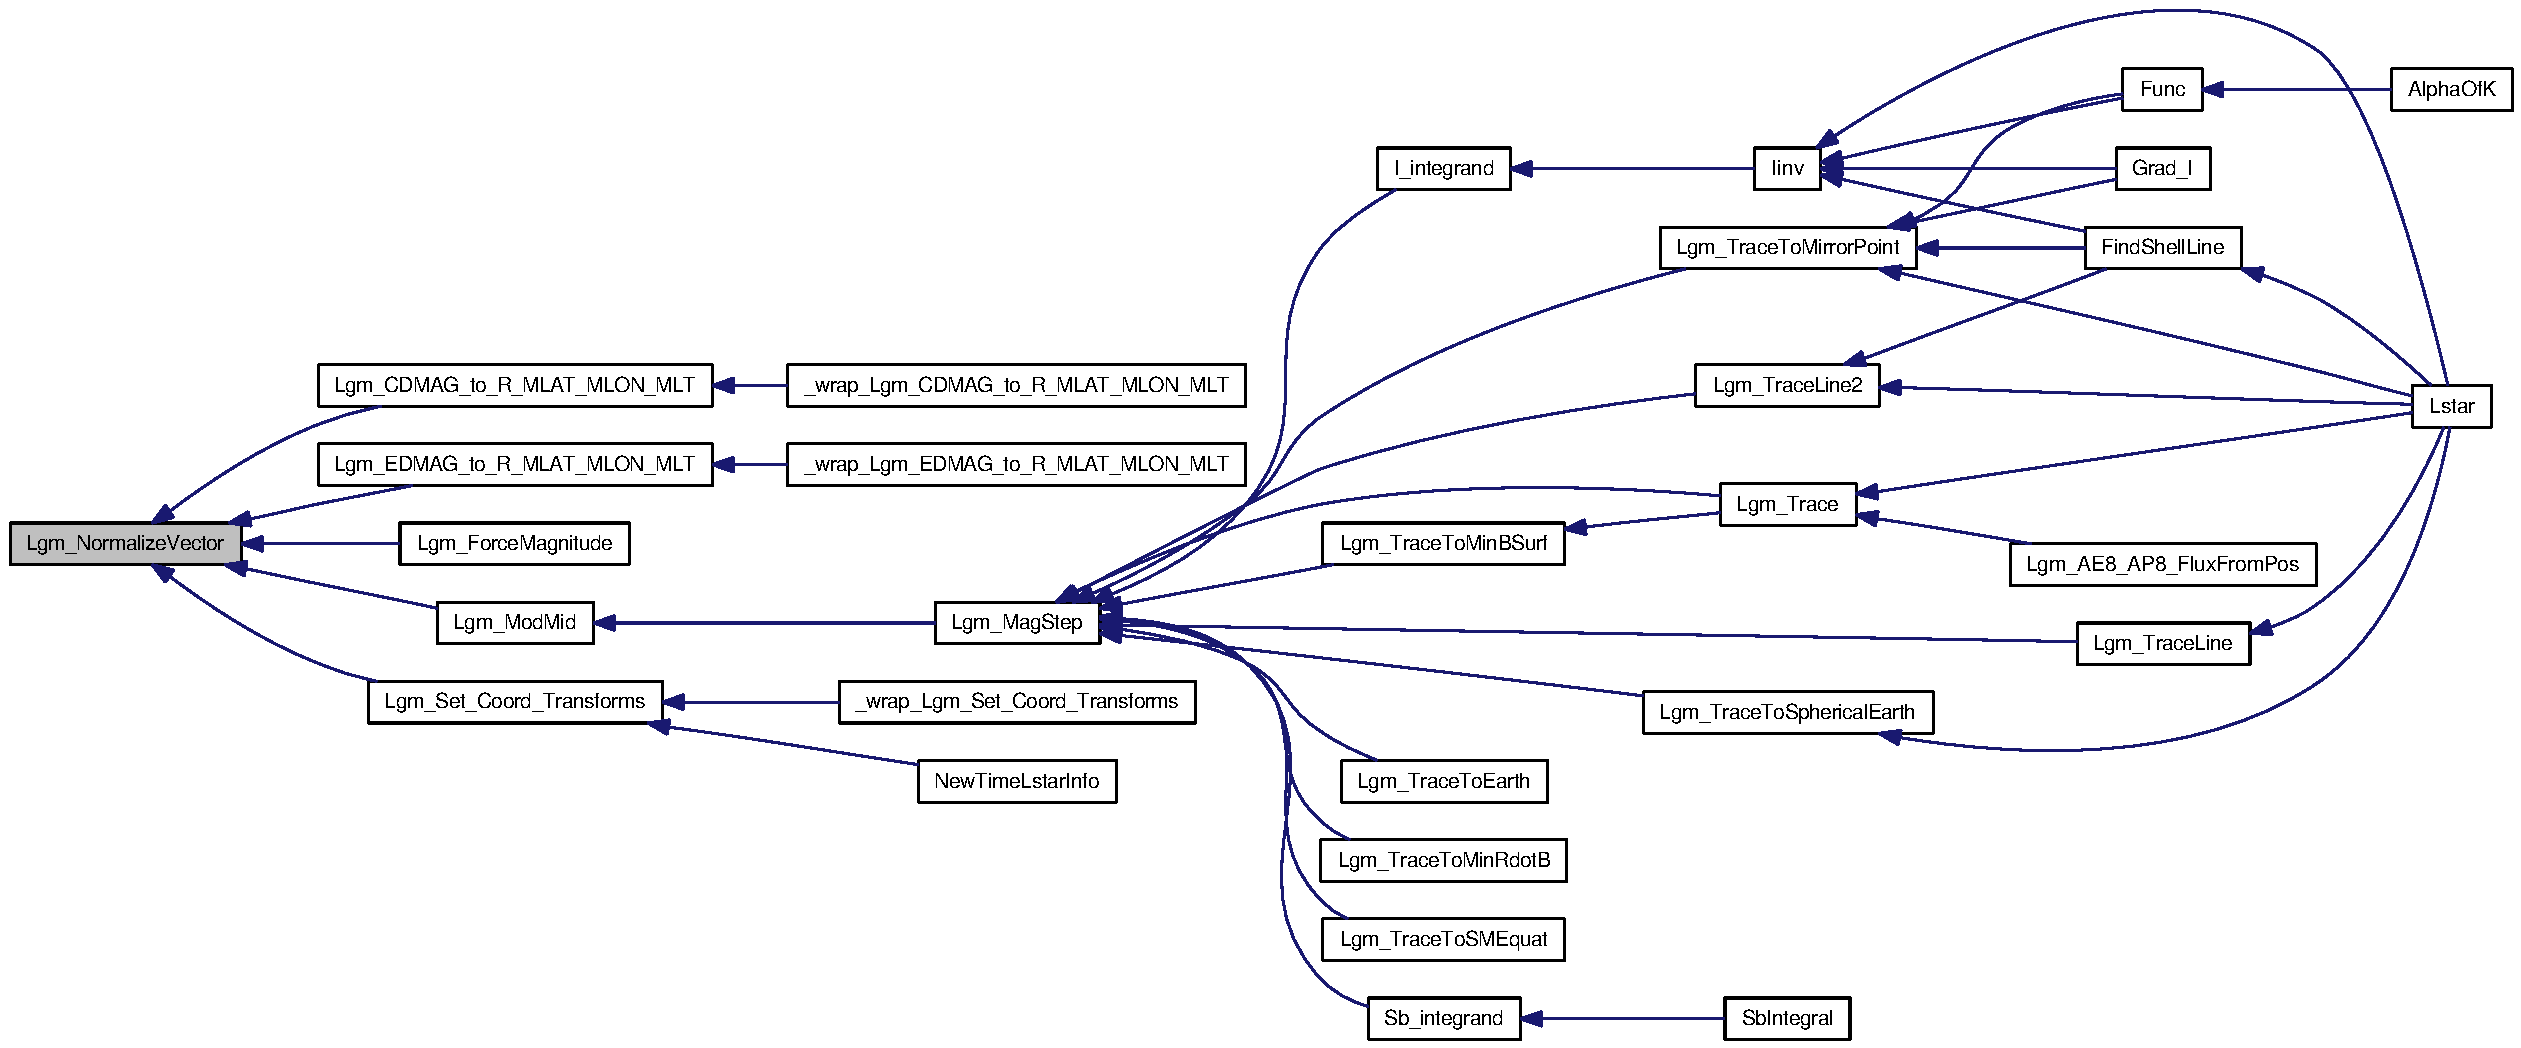
\includegraphics[width=420pt]{vec_8c_851c60a1429e5b2d8bc5feb2d59af700_icgraph}
\end{center}
\end{figure}
\hypertarget{vec_8c_eb74ea961a602bfdb729ade5b1282946}{
\index{vec.c@{vec.c}!Lgm\_\-ScaleVector@{Lgm\_\-ScaleVector}}
\index{Lgm\_\-ScaleVector@{Lgm\_\-ScaleVector}!vec.c@{vec.c}}
\subsubsection[{Lgm\_\-ScaleVector}]{\setlength{\rightskip}{0pt plus 5cm}void Lgm\_\-ScaleVector ({\bf Lgm\_\-Vector} $\ast$ {\em a}, \/  double {\em value})}}
\label{vec_8c_eb74ea961a602bfdb729ade5b1282946}




Definition at line 46 of file vec.c.

Here is the caller graph for this function:\nopagebreak
\begin{figure}[H]
\begin{center}
\leavevmode
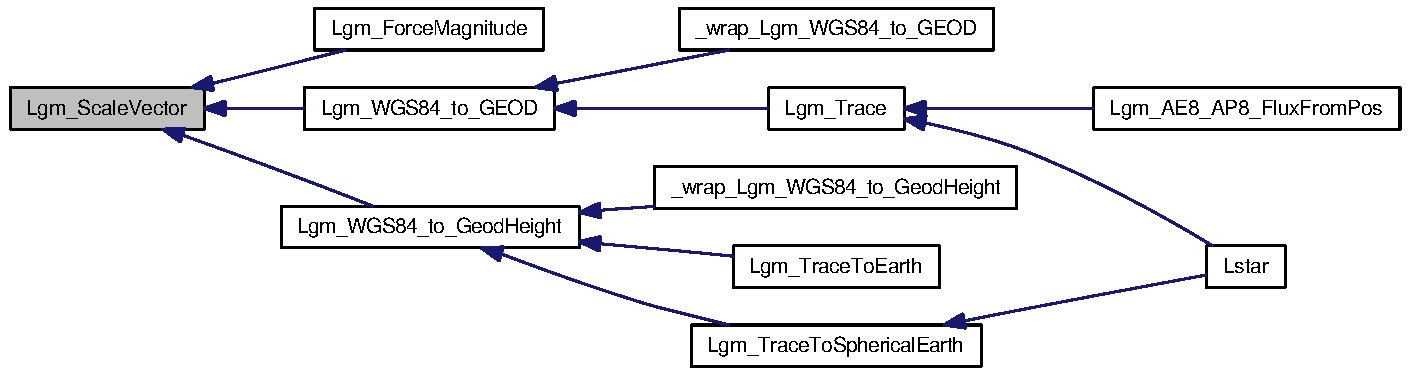
\includegraphics[width=356pt]{vec_8c_eb74ea961a602bfdb729ade5b1282946_icgraph}
\end{center}
\end{figure}
\hypertarget{vec_8c_84b4b9aa2d74211cb12654e6be70cb82}{
\index{vec.c@{vec.c}!Lgm\_\-Magnitude@{Lgm\_\-Magnitude}}
\index{Lgm\_\-Magnitude@{Lgm\_\-Magnitude}!vec.c@{vec.c}}
\subsubsection[{Lgm\_\-Magnitude}]{\setlength{\rightskip}{0pt plus 5cm}double Lgm\_\-Magnitude ({\bf Lgm\_\-Vector} $\ast$ {\em a})}}
\label{vec_8c_84b4b9aa2d74211cb12654e6be70cb82}




Definition at line 56 of file vec.c.

Here is the caller graph for this function:\nopagebreak
\begin{figure}[H]
\begin{center}
\leavevmode
\includegraphics[width=420pt]{vec_8c_84b4b9aa2d74211cb12654e6be70cb82_icgraph}
\end{center}
\end{figure}
\hypertarget{vec_8c_47c6f330f5c1228f812b005094b64dfd}{
\index{vec.c@{vec.c}!Lgm\_\-ForceMagnitude@{Lgm\_\-ForceMagnitude}}
\index{Lgm\_\-ForceMagnitude@{Lgm\_\-ForceMagnitude}!vec.c@{vec.c}}
\subsubsection[{Lgm\_\-ForceMagnitude}]{\setlength{\rightskip}{0pt plus 5cm}void Lgm\_\-ForceMagnitude ({\bf Lgm\_\-Vector} $\ast$ {\em a}, \/  double {\em mag})}}
\label{vec_8c_47c6f330f5c1228f812b005094b64dfd}




Definition at line 64 of file vec.c.

Here is the call graph for this function:\nopagebreak
\begin{figure}[H]
\begin{center}
\leavevmode
\includegraphics[width=151pt]{vec_8c_47c6f330f5c1228f812b005094b64dfd_cgraph}
\end{center}
\end{figure}
\hypertarget{vec_8c_d6b4ead73e36f4f3f77cc62bc88555d3}{
\index{vec.c@{vec.c}!Lgm\_\-MatTimesVec@{Lgm\_\-MatTimesVec}}
\index{Lgm\_\-MatTimesVec@{Lgm\_\-MatTimesVec}!vec.c@{vec.c}}
\subsubsection[{Lgm\_\-MatTimesVec}]{\setlength{\rightskip}{0pt plus 5cm}void Lgm\_\-MatTimesVec (double {\em A}\mbox{[}3\mbox{]}\mbox{[}3\mbox{]}, \/  {\bf Lgm\_\-Vector} $\ast$ {\em V}, \/  {\bf Lgm\_\-Vector} $\ast$ {\em Result})}}
\label{vec_8c_d6b4ead73e36f4f3f77cc62bc88555d3}




Definition at line 76 of file vec.c.

Here is the caller graph for this function:\nopagebreak
\begin{figure}[H]
\begin{center}
\leavevmode
\includegraphics[width=420pt]{vec_8c_d6b4ead73e36f4f3f77cc62bc88555d3_icgraph}
\end{center}
\end{figure}
\hypertarget{vec_8c_2afeb786399b91dc38ba78adc88db1ce}{
\index{vec.c@{vec.c}!Lgm\_\-MatTimeMat@{Lgm\_\-MatTimeMat}}
\index{Lgm\_\-MatTimeMat@{Lgm\_\-MatTimeMat}!vec.c@{vec.c}}
\subsubsection[{Lgm\_\-MatTimeMat}]{\setlength{\rightskip}{0pt plus 5cm}void Lgm\_\-MatTimeMat (double {\em A}\mbox{[}3\mbox{]}\mbox{[}3\mbox{]}, \/  double {\em B}\mbox{[}3\mbox{]}\mbox{[}3\mbox{]}, \/  double {\em Result}\mbox{[}3\mbox{]}\mbox{[}3\mbox{]})}}
\label{vec_8c_2afeb786399b91dc38ba78adc88db1ce}




Definition at line 88 of file vec.c.